\documentclass[12pt, letter]{exam}
\usepackage[utf8]{inputenc}
\usepackage[T1]{fontenc}
\usepackage[spanish]{babel}
\usepackage[autostyle,spanish=mexican]{csquotes}
\usepackage{amsmath}
\usepackage{amsthm}
\usepackage{physics}
\usepackage{tikz}
\usepackage{float}
\usepackage{siunitx}
\usepackage{multicol}
\usepackage[left=2.00cm, right=2.00cm, top=2.00cm, 
     bottom=2.00cm]{geometry}
\usepackage{pdfpages}

% \renewcommand{\questionlabel}{\thequestion}
\decimalpoint

\setlength{\belowdisplayskip}{-0.5pt}

\usepackage{tasks}
\settasks{
    label=\Alph*), 
    label-align=left,
    item-indent={20pt}, 
    column-sep={4pt},
    label-width={16pt},
}

\sisetup{per-mode=symbol}
\footer{}{\thepage}{}

\begin{document}
\includepdf[pages={1}]{Caratula_Examen_Parcial_02_PU_Fisica_4_03.pdf}

\newpage

\begin{questions}
    
    \section{Naturaleza de la luz.}
    
    \question Nombre del científico que propuso que la luz está constituida por numerosos corpúsculos o partículas emitidas por cualquier cuerpo luminoso
    \begin{tasks}(4)
        \task James \\ Maxwell.
        \task Willebrord \\ Snell.
        \task Isaac \\ Newton.
        \task Christian \\ Huygens.
    \end{tasks}
    \question ¿Cuáles son las características de la luz que se cumplen tanto en la teoría corpuscular de la luz y la teoría ondulatoria?
    \begin{parts}
        \part Refracción, Reverberación, Reflexión.
        \part Propagación rectilínea, Reflexión, Refracción.
        \part Reflexión, Resonancia, Propagación rectilínea.
        \part Refracción, Efecto Doppler, Reflexión.
    \end{parts}
    \question Completa la frase con la palabra que hace falta. Un cuepo \rule{2cm}{0.1mm} permite el paso de los rayos luminosos, por lo que se ve con claridad cualquier objeto colocado al otro lado de él.
    \begin{tasks}(4)
        \task Reflejante.
        \task Opaco.
        \task Transparente.
        \task Translúcido.
    \end{tasks}
    
    \section{Óptica geométrica.}

    \question De la ley de Snell se nos pide obtener el ángulo $b$ (incidente), ¿cuál es la expresión que nos resuelve el problema?
    \begin{tasks}
        \task $ b = \sen^{-1} \left(\dfrac{n_{b} \, \text{sen} \, a}{n_{a}} \right)$
        \task $ b = \sen^{-1} \left(\dfrac{n_{a} \, \text{sen} \, a}{n_{b}} \right)$
        \task $ b = \sen^{-1} \left(\dfrac{n_{a} \, n_{b}}{\text{sen} \, a} \right)$
        \task $ b = \sen^{-1} \left(\dfrac{\text{sen} \, a}{n_{a} \, n_{b}} \right)$
    \end{tasks}
    \question La refracción de la luz consiste en la desviación que sufren los rayos luminosos cuando llegan a la superficie de separación entre dos sustancias o medios de diferente \rule{2.5cm}{0.1mm}.
    \begin{tasks}(4)
        \task Peso.
        \task Volumen.
        \task Densidad.
        \task Grosor.
    \end{tasks}
    \question \label{Problema_01} \textbf{Ejercicio de ejecución: } El haz de una linterna incide sobre la superficie de un panel de vidrio $(n = 1.56)$ en un ángulo de \ang{75} con la normal. ¿Cuál es el ángulo de refracción?
    \begin{tasks}(4)
        \task \ang{39;49;51}
        \task \ang{38;15;23}
        \task \ang{48;4;36}
        \task \ang{27;11;58}
    \end{tasks}
    \question Tomando el enunciado anterior de la linterna, ahora considera que el haz de luz incide sobre la superficie de otro material cuyo índice es $n_{2} = 1.7$, en comparación al ángulo de refracción con el vidrio $\theta_{n1}$, ¿cómo será el ángulo de refracción $\theta_{n2}$ en la otra superficie?
    \begin{tasks}(4)
        \task Mayor que $\theta_{n1}$
        \task Menor que $\theta_{n1}$
        \task Son iguales.
        \task La mitad de $\theta_{n1}$
    \end{tasks}
    

    \section{Lentes delgadas.}

    \question Las lentes \rule{2.5cm}{0.1mm} son aquellas cuyo espesor disminuye de los bordes hacia el centro, hablamos de las lentes:
    \begin{tasks}(4)
        \task Esféricas.
        \task Divergentes.
        \task Convergentes.
        \task Cilíndricas.
    \end{tasks}
    \question Cuando hablamos del punto donde se cruzan los rayos que llegan a la lente en forma paralela al eje principal, estamos hablando de:
    \begin{tasks}(4)
        \task Centro \\ geométrico.
        \task Plano \\ central
        \task Foco \\ principal.
        \task Eje \\ principal.
    \end{tasks}
    \question La propiedad del centro óptico de la lente nos dice que en ese punto la desviación de un rayo de luz es:
    \begin{tasks}(4)
        \task Infinita.
        \task Perpendicular al \\ eje principal.
        \task Nula.
        \task Máxima.
    \end{tasks}
    \question Revisa con cuidado la siguiente imagen e identifica las siguientes lentes.
    \begin{figure}[H]
        \centering
        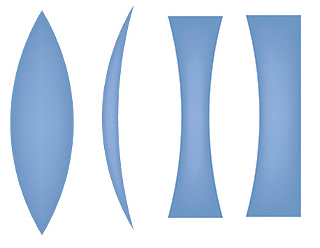
\includegraphics[scale=2]{Imagenes/Arreglo_Lentes_02.png}
    \end{figure}
    \begin{tasks}(4)
        \task +, - , +, - 
        \task -, - , +, + 
        \task +, + , -, - 
        \task -, + , -, + 
    \end{tasks}
    \question De la convención de signos para las lentes delgadas:  La distancia del objeto $d_{i}$ es \rule{2cm}{0.1mm} si el objeto está en el lado contrario de la lente de donde proviene la luz:
    \begin{tasks}(4)
        \task Positiva.
        \task Cero.
        \task Negativa.
        \task Infinita.
    \end{tasks}
    \question De la convención de signos para las lentes delgadas:  La distancia de la imagen $d_{i}$ es \rule{2cm}{0.1mm} para una imagen real.
    \begin{tasks}(4)
        \task Positiva.
        \task Negativa.
        \task Infinita.
        \task Cero.
    \end{tasks}
    \question \label{Problema_02} \textbf{Ejercicio de ejecución. } Un objeto de \SI{15}{\centi\meter} se coloca a \SI{50}{\centi\meter} de una lente positiva que tiene una distancia focal de \SI{20}{\centi\meter}. ¿De qué tamaño es la imagen?
    \begin{tasks}(4)
        \task \SI{35}{\centi\meter}
        \task \SI{10}{\centi\meter}
        \task \SI{25}{\centi\meter}
        \task \SI{5}{\centi\meter}
    \end{tasks}
    \question \label{Problema_03} \textbf{Ejercicio de ejecución: } ¿Cuál es la potencia de una lente con \SI{15}{\centi\meter} de distancia focal?
    \begin{tasks}(4)
        \task \num{-2.98} Dioptrías
        \task \num{2.98} Dioptrías
        \task \num{6.66} Dioptrías
        \task \num{-5.25} Dioptrías
    \end{tasks}

    \section{El ojo y la visión.}

    \question El siguiente esquema representa un ojo humano, ¿cómo se denomina al caso en términos de anomalías/normalidad de la visión?
    \begin{figure}[H]
        \centering
        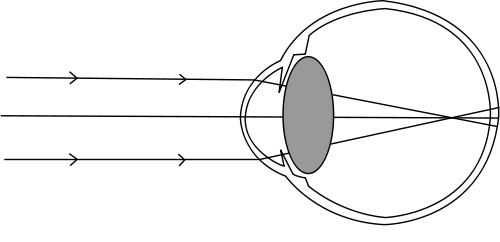
\includegraphics[scale=0.3]{Imagenes/Defectos_Vision_03.png}
    \end{figure}
    \begin{tasks}(4)
        \task Ojo astigmata.
        \task Ojo emétrope.
        \task Ojo hipermétrope.
        \task Ojo miope.
    \end{tasks}
    \question El ojo présbita: suele ser un ojo \enquote{cansado} debido a que la facultad de \rule{2cm}{0.1mm} ha disminuido.
    \begin{tasks}(4)
        \task Acomodación \\ del cristalino.
        \task Visión binocular.
        \task Densidad del \\ humor vítreo.
        \task Presión interna.
    \end{tasks}
    \question El siguiente esquema representa en términos de anomalías/normalidad de la visión?
    \begin{figure}[H]
        \centering
        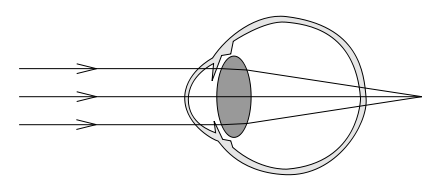
\includegraphics[scale=0.4]{Imagenes/Defectos_Vision_05.png}
    \end{figure}
    \begin{tasks}(4)
        \task Ojo hipermétrope.
        \task Ojo astigmata.
        \task Ojo emétrope.
        \task Ojo miope.
    \end{tasks}
    \question  La \rule{2cm}{0.1mm} es la capacidad de utilizar ambos ojos de manera coordinada y simultánea para percibir una sola imagen tridimensional del entorno.
    \begin{tasks}(4)
        \task Visión periférica.
        \task Visión 20/20.
        \task Visión monocular.
        \task Visión binocular.
    \end{tasks}
    \question Cuando decimos que se trata de una enfermedad degenerativa provocada por la alteración en las fibras de colágeno que componen el estroma (la parte más gruesa de la córnea), provocando una pérdida paulatina de la visión. Hablamos de:
    \begin{tasks}(4)
        \task Cataratas.
        \task Glaucoma.
        \task Queratocono.
        \task Escotoma.
    \end{tasks}
\end{questions}

\newpage

\textbf{\huge{Formulario.}}
\begin{table}[H]
    \centering
    \setlength{\tabcolsep}{40pt}
    \renewcommand{\arraystretch}{2.5}
    \begin{tabular}{c  c}
        \multicolumn{2}{c}{Óptica geométrica} \\
        $n = \dfrac{\text{sen} \, i}{\text{sen} \, i}$ & $n_{a} \, \text{sen} \,  a = n_{b} \, \text{sen} \,  b$ \\ \hline
        \multicolumn{2}{c}{Lentes delgadas} \\
        $\dfrac{1}{f} = \dfrac{1}{d_{o}} + \dfrac{1}{d_{i}}$ (lente convergente) & $- \dfrac{1}{f} = \dfrac{1}{d_{o}} - \dfrac{1}{d_{i}}$ (lente divergente) \\
        $m = - \dfrac{d_{i}}{d_{o}} = \dfrac{h_{i}}{h_{o}}$ & $\text{Potencia } = \dfrac{1}{f} \quad f \text{ en } \unit{\meter}$ \\ \hline
\end{tabular}
\end{table}

En este espacio deberás de incluir el desarrollo completo de los Problemas de Ejecución. Recuerda que si no se tiene el desarrollo, el problema no aportará puntaje aunque se tenga la respuesta correcta.

\vspace*{0.5cm}
Solución al Problema de Ejecución \ref{Problema_01}:

\vspace*{4cm}
\rule{0.9\textwidth}{0.3mm}

Solución al Problema de Ejecución \ref{Problema_02}:

\vspace*{4.5cm}
\rule{0.9\textwidth}{0.3mm}

Solución al Problema de Ejecución \ref{Problema_03}:


\end{document}